\chapter{Results}
Simulating real applications in virtual hardware without any real interaction is hard and there are many things that can break along the way. The simulations were run on a by Chalmers provided compute cluster and took quite some time to complete. This cluster luckily used an older version of Ubuntu with a relatively old kernel, and since PIN 2 depends on older kernel functionality it meant it could be run without a hitch. In addition, in order to support the old ABI used with some of its binaries while having full support for C++11, GCC 4.9.4 had to be used, specifically. 
\bigskip

In this chapter we will first measure what latency behaviour looks like when using one single HMC device, with a single link hop. Then we will increase the number of devices and always use the device at the end of the chain, e.g. when having 8 devices we will perform all allocations on the 8th device. We will view these results both from a device and a application perspective. Finally, we present a short summary of our findings.

\section{Simulation}
The simulations were run with multiple configurations, where every application (stated in TODO: ref) was run with either 4 or 8 links configured, enabling between 1 and 6 memory cubes and data was allocated on the last memory unit in the network. The reason for testing both 4 and 8 links was to see whether the increased bandwidth, and in this case amount of parallelism, would significantly impact the latencies. 
\bigskip

A first test was run with 429.mcf, which is arguably the most memory intense and latency sensitive benchmark out of the chose applications, just to see how the system's simulated memory would behave. This test was run using one active link and data allocated on the closest device. Figure \ref{Memory-access-behaviour} shows a graph over the number of times a specific access time, in ns, was reached for all simulated memory requests. The pattern seen is a more or a less repetitive form which reappears with 93 ns interval. The single link means that we only are connected directly to a single vault, and accesses to memory locations belonging to other vaults will have to be routed in the mesh network. However, since HMCSim probably does not perform a DRAM lookup -- which would incur a 93 ns latency, given our configuration -- for a request not belonging to the single vault, it is more likely that this pattern is due to HMC's Custom Memory Commands (CMC). A few such are implemented in HMCSim, e.g. for atomic access to multiple pages, and these will perform a new lookup for every requested page. The high amount of latency this adds is most likely due to HMC using a closed page policy, meaning that there will be no hits in the row buffer and even sequential data will have to fetched again.

\begin{figure}[!h]
\centering
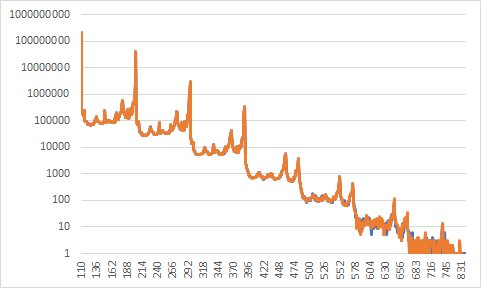
\includegraphics[width=0.75\linewidth]{figure/Testdata-4dev-4or1link-alloc0.png}
\caption{Number of occurrences for different memory access times. }
\label{Memory-access-behaviour}
\end{figure}

\section{Summary}
Summarise the results without actually discussing the implications; leave that for the next part!